% !TEX root = ../main.tex

\chapter{Patanalysis}
\label{ch:analysis}

\startcontents[chapters]

Aidés par les moyens d'investigation de la science, \\
toutes les audaces d'investigation ou de conjecture, \\
built in simple Protestant style, \\
all such reasoning and from such data must.

And I style him friend, \\
its whole style differed materially from that of Legrand, \\
the calculus of Probabilities, \\
n'échappaient à leur investigation.

Another line of reasoning partially decided me, \\
to make an anatomical dissection of its body and, \\
ce style en débâcle et innavigable.

In a style Of gold, \\
que la sobriété du style se conduit de la sorte, \\
still a point worthy very serious investigation.

\minicontents

\section{Problems Encountered}

% \begin{draft}
%   \section{User experience}
%
%   Whilst developing a system that returns creative results to the end user has numerous advantages, the assumptions that are made about and the decisions we take for the user must still be considered. For example, presume that the user inputs a search request `The Cat in the Hat' after reading a Dr.\ Seuss book to their child, and the system employs an anomalous method on the query and searched `sunglasses'. Whilst there is logic to the new search request, it is anomalous to the initial request, if the user receives these results without being told what method was used, the results will appear random, and therefore are likely to be detrimental to the user. Therefore the level of interaction the user has with the system and the feedback the system gives to the user on decisions it is making will have a large influence on the overall effectiveness and appreciation of the search tool. A quick and simple solution to this problem would be to add an icon to the side of each search result which displays how the original query was pataphysicalised.
%
%   \begin{figure}[htb] % (here, top, bottom, page)
%     \centering
%     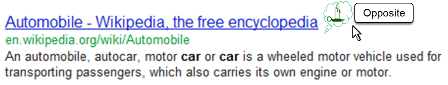
\includegraphics[width=\linewidth]{images/resultexample}
%   \caption[Feedback button]{Feedback button}
%   \label{fig:feedback}
%   \end{figure}
%
%   The above image (figure~\ref{fig:feedback}) shows an example of how this could be implemented. The little green candle (a reference to pataphysics in itself by the way) shows a pop-up note when hovered over with the mouse pointer. In this case the original query could have been `tree' and `car' was returned as an opposite to that.
% \end{draft}


\section{Design Aspects}

\section{Search Results}

\stopcontents[chapters]
